%TCIDATA{LaTeXparent=0,0,relatorio.tex}



\chapter{Resultados\label{chap:Resultados}}

% Resumo opcional. Comentar se não usar.
\resumodocapitulo{``Analisar os dados tops!'' -- Tiago}


\section{Introdução}

Nesse capítulo iremos mostrar os resultados dos experimentos realizados, descritos na seção \ref{section:TestesRealizados}. Vamos também analisar esses resultados.

Breve explicação dos experimentos que permitiram esses resultados.
Qual o setup? Quais os valores dos parâmetros? Qual o experimento,
qual era o objetivo desse experimento?


\section{Resultados}

Resultados obtidos com o trabalho e a análise quantitativa e qualitativa
em forma de gráficos, imagens e números.

\subsection{3 Comportamentos no mapa pequeno (Teste 1)}

Esse experimento está descrito no tópico \ref{subsection:3ComportamentosMapaPequeno}.

Os valores dos pesos $ \omega $ evoluiram segundo os seguintes gráficos:

\begin{figure}[H]
    \centering
    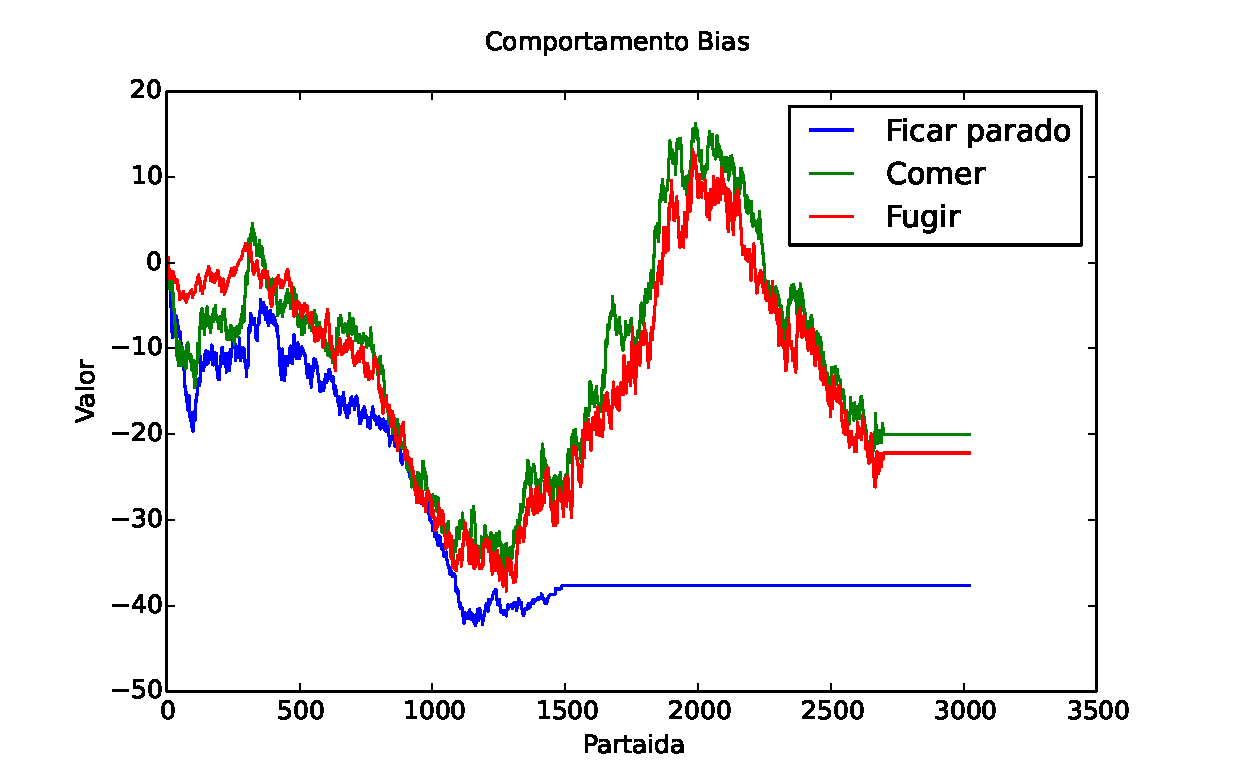
\includegraphics[width=120mm]{images/3_behaviors_small_map/weights____pol__Bias}
    \caption{\label{img:3ComportamentosMapaPequeno:ComportamentoParar}Evolução dos pesos $ \omega $ do comportamento parar.}
\end{figure}

\begin{figure}[H]
    \centering
    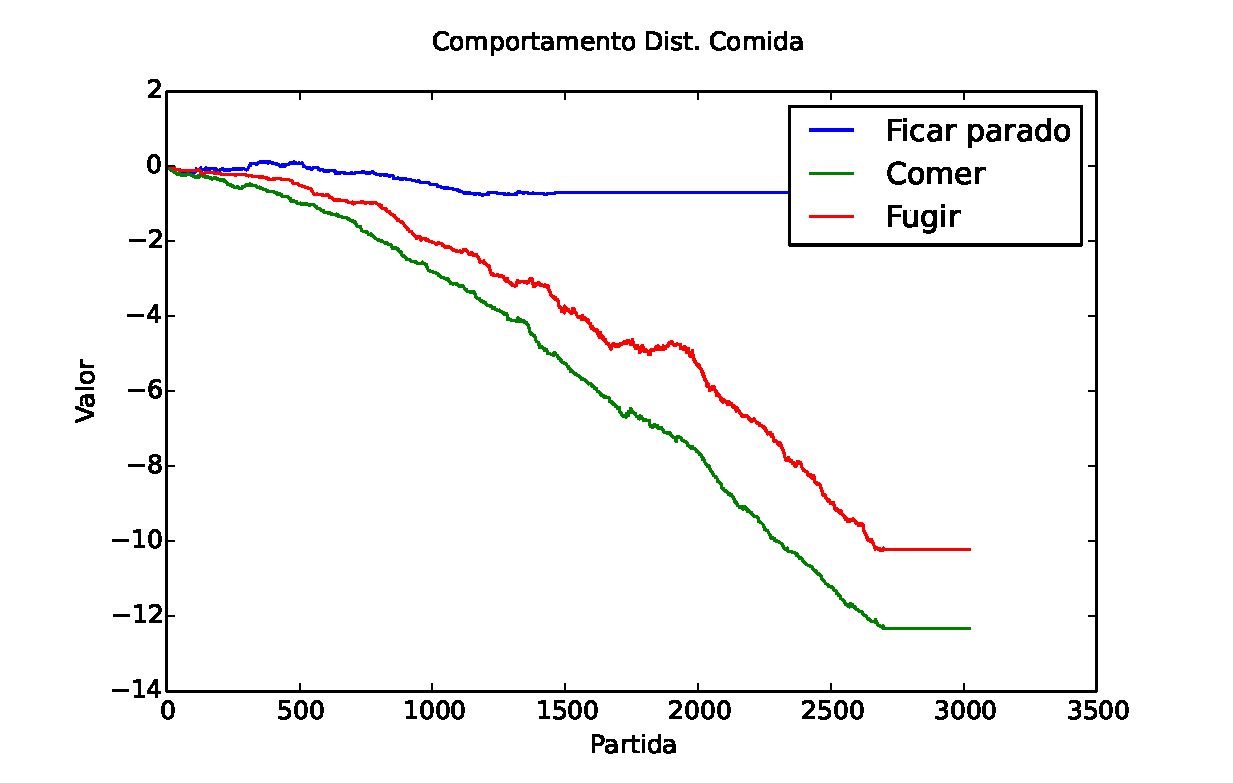
\includegraphics[width=120mm]{images/3_behaviors_small_map/weights____pol__DistComida}
    \caption{\label{img:3ComportamentosMapaPequeno:ComportamentoComer}Evolução dos pesos $ \omega $ do comportamento comer.}
\end{figure}

\begin{figure}[H]
    \centering
    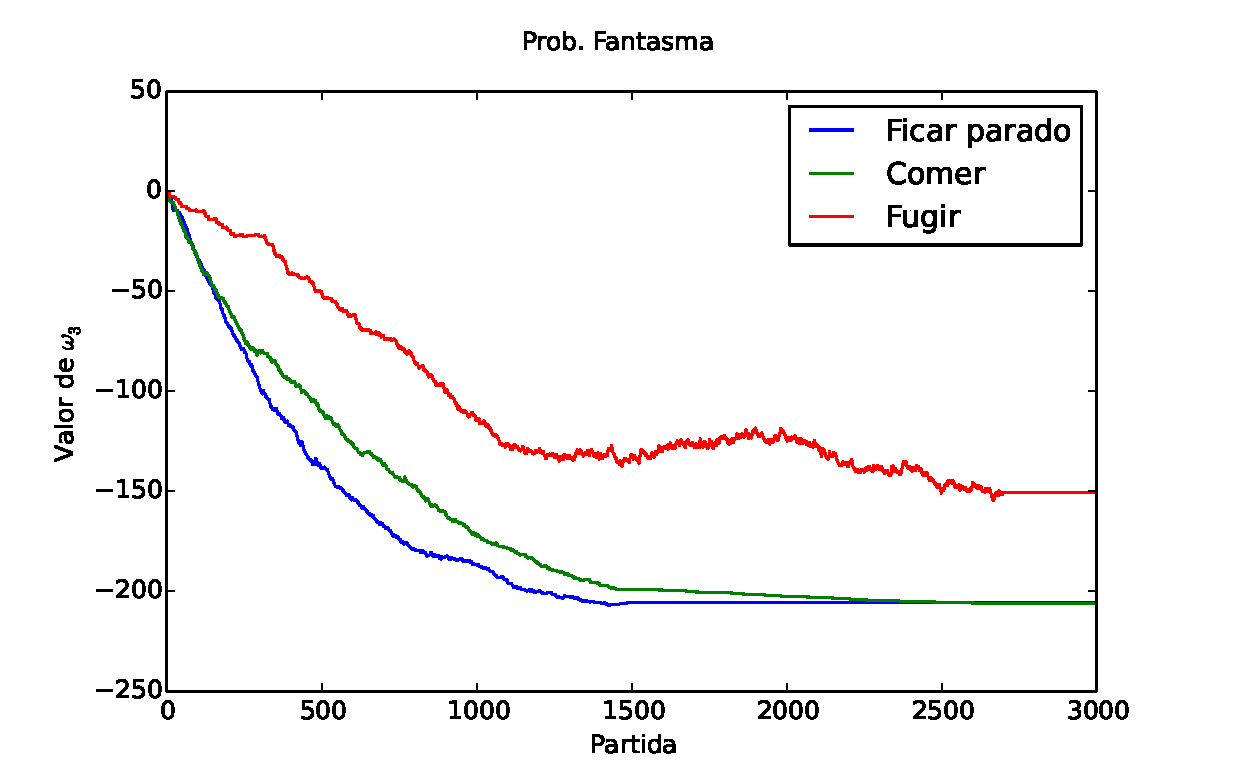
\includegraphics[width=120mm]{images/3_behaviors_small_map/weights____pol__ProbFantasma}
    \caption{\label{img:3ComportamentosMapaPequeno:ComportamentoFugir}Evolução dos pesos $ \omega $ do comportamento fugir.}
\end{figure}


Os comportamentos escolhidos ao longo do tempo formam a seguinte nuvem:

\begin{figure}[H]
    \centering
    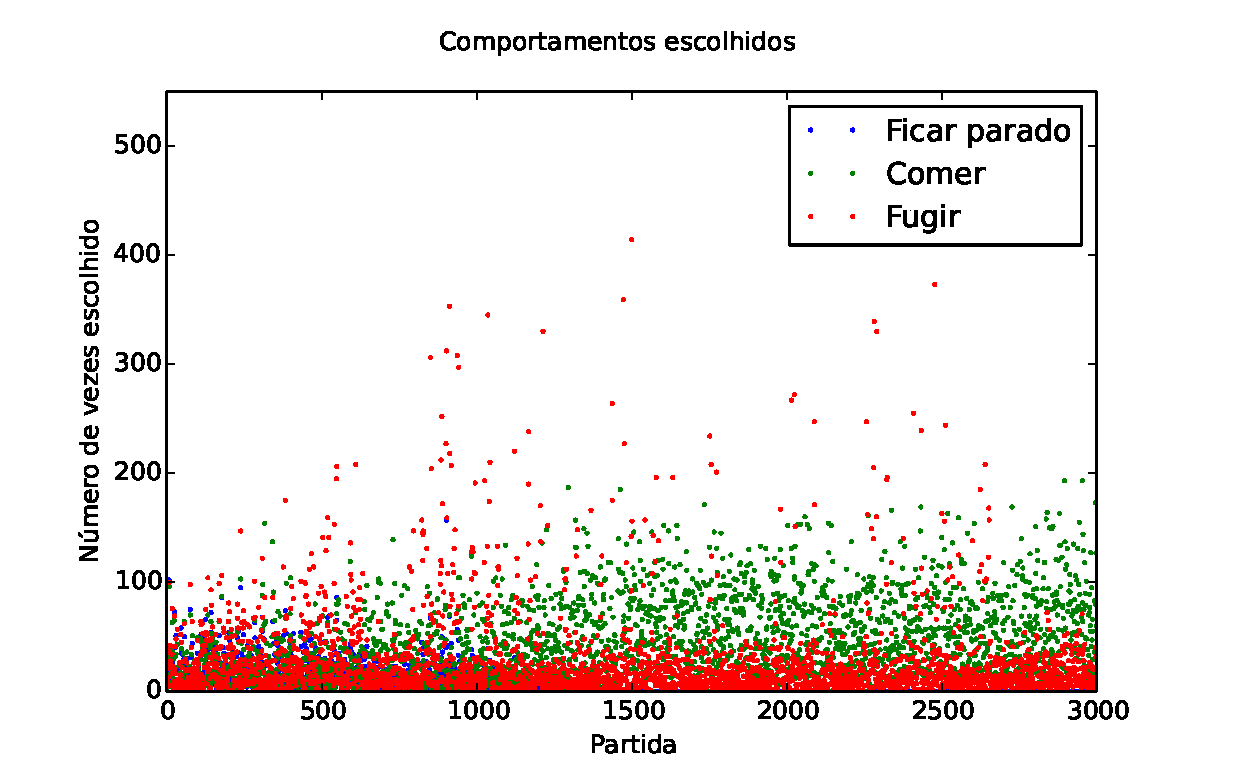
\includegraphics[width=170mm]{images/3_behaviors_small_map/chosen_behaviors}
    \caption{\label{img:3ComportamentosMapaPequeno:ComportamentosEscolhidos}Escolha de comportamentos por partida.}
\end{figure}

Que, ao ser aproximada por um polinômio de terceiro grau forma a seguinte curva:

\begin{figure}[H]
    \centering
    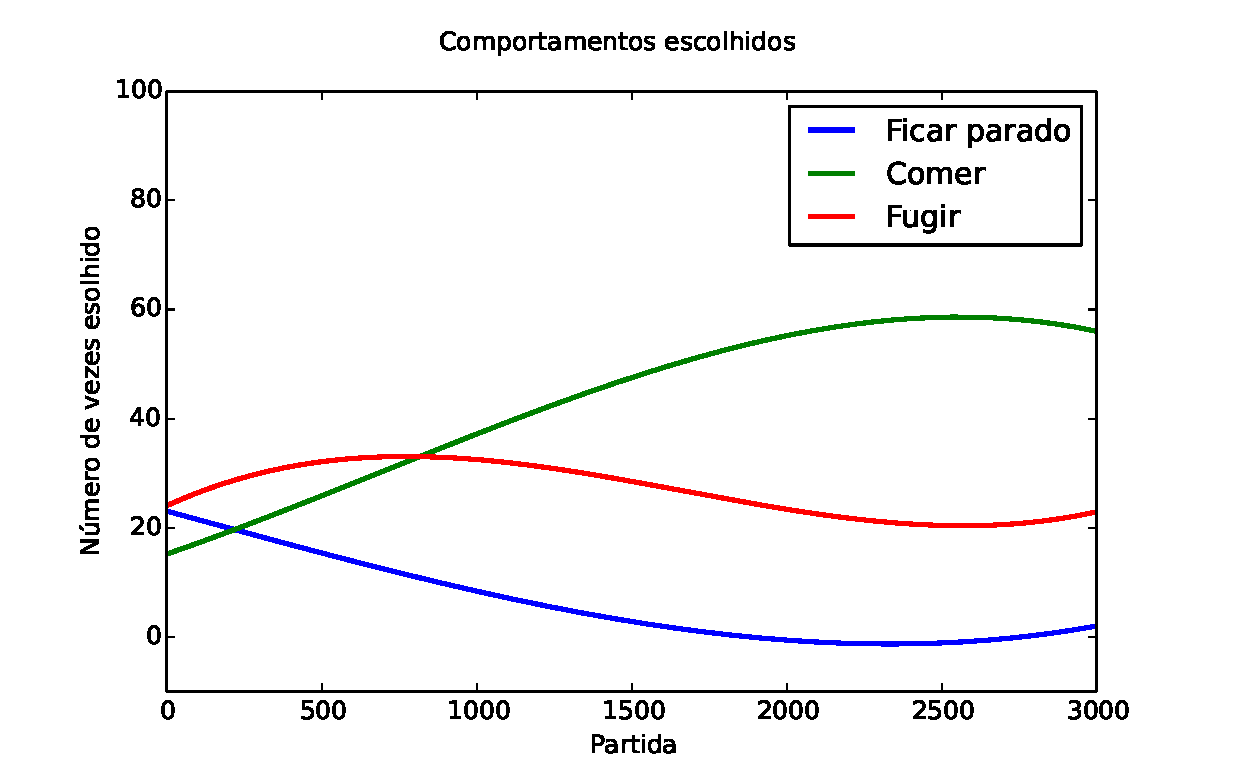
\includegraphics[width=170mm]{images/3_behaviors_small_map/chosen_behaviors_pol}
    \caption{\label{img:3ComportamentosMapaPequeno:ComportamentosEscolhidosPolinômio}Escolha de comportamentos por partida.}
\end{figure}

A pontuação ao final das partidas forma a seguinte novem:

\begin{figure}[H]
    \centering
    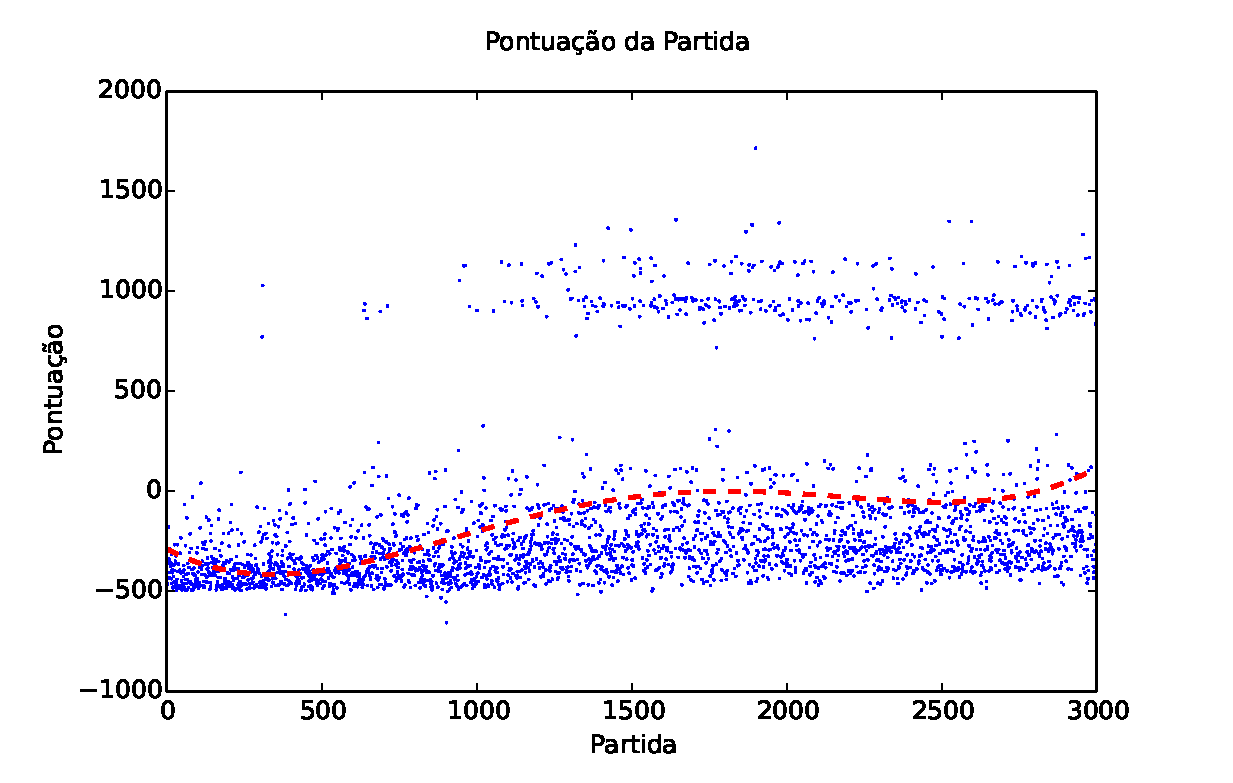
\includegraphics[width=170mm]{images/3_behaviors_small_map/match_scores____pol}
    \caption{\label{img:3ComportamentosMapaPequeno:PontuacaoPorPartida}Escolha de comportamentos por partida.}
\end{figure}

E pode ser aproximada pelo seguinte polinômio de quarto grau:


\subsection{3 Comportamentos no mapa original (Teste 2)}
\subsection{5 Comportamentos no mapa pequeno (Teste 3)}
\subsection{5 Comportamentos no mapa original (Teste 4)}
